\documentclass{article}

\usepackage[utf8]{inputenc} % For Unicode characters
\usepackage{amsmath}        % For mathematical symbols
\usepackage{graphicx}       % For including images
\usepackage{hyperref}       % For hyperlinks
\usepackage{geometry}      % For setting page margins
\usepackage{float}
\usepackage{tcolorbox}
\usepackage{tikz}

% Set the page margins
\geometry{margin=1in}
% Set the top margins
\addtolength{\topmargin}{-.5in}

\title{Engineering Optics, Homework 3}
\author{He Tianyang}
\date{\today}


\begin{document}

\maketitle

\section{Problem 1}
\textbf{Chapter 3, Problem 3}\\\\

The optical leaver follows the following equation:
\begin{equation}
    y = x\cdot\frac{2f'}{a}
\end{equation}

where $f'$ is the focal length of the lens, $a$ is the distance between the axis and the test rod, and $x$ is the distance between the mirror and the original position.

Given that $f' = 1000\textbf{mm}$, $a = 10\textbf{mm}$, and $y = 2\textbf{mm}$, we can calculate the displacement x;

\begin{equation}
    x = \frac{y\cdot a}{2f'} = \frac{2\cdot 10}{2\cdot 1000} = 0.02\textbf{mm}
\end{equation}

Therefore, the mirror rotates by $0.02\textbf{mm}$. the angle of rotation is given by:

\begin{equation}
    \theta = \arcsin{\frac{x}{a}} = \arcsin{\frac{0.02}{10}} \approx 0.114591635420675 \textbf{rad}
\end{equation}

To summarize, the mirror rotates by $\mathbf{0.02}\textbf{mm}$, and the angle of rotation is $\mathbf{0.114591635420675}\textbf{rad}    $.

\section{Problem 2}
\textbf{Chapter 3, Problem 7}\\\\

The answer is given in the Figure \ref{fig:3-7} and marked with boxed.

\begin{figure}[H]
    \centering
    \includegraphics[width=0.7\textwidth]{./image/hw3/hw3_1.jpeg}
    \caption{Chapter 3, Problem 7}
    \label{fig:3-7}
\end{figure}

\section{Problem 3}
\textbf{Chapter 3, Problem 13}\\\\

The Optical Wedge follows the following equation:
\begin{equation}
    \delta = \left(n\cdot\frac{\cos{I_1'}}{\cos{I_1}} - 1\right)\alpha
\end{equation}

where $\delta$ is the deviate angle, $n$ is the refractive rate of the wedge, $I_1$ is the angle of incidence, $I_1'$ is the angle of refraction, and $\alpha$ is the angle of the wedge.

In this case, $I_1$ and $I_1'$ are small enough, so we have
\begin{equation}
    \delta = (n-1)\alpha = (1.5163-1)\cdot 4^{\circ} = 0.20652^{\circ}
\end{equation}

Therefore, the incidence ray deviates by $\mathbf{0.20652^{\circ}}$. to accomplish the same deviation, the mirror should  rotates by $\theta$, where:
\begin{equation}
    \boxed{
        \theta = \frac{\alpha}{2} = 0.10326^{\circ}
    }
\end{equation}

\section{Problem 4}
\textbf{Chapter 3, Problem 17}\\\\

When passing a mirror, the $y$ axis is always perpendicular to the mirror, the $z$ axis is always parallel to the axis, and the $x$ axis will be reversed.

When passing a lens, the $z$ axis is still parallel to the axis, but the $x$ and $y$ axis will be reversed.


In this case, after passing the $P_1$, the $x$ axis is reversed, so the coordinate system is shown in Figure \ref{fig:3-17-1}.

\begin{figure}[H]
    \centering
    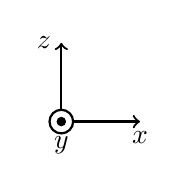
\begin{tikzpicture}
        % Draw axes
        \draw[thick,->] (1.5mm,0) -- (1,0) node[anchor=north]{$x$};
        \draw[thick,->] (0,1.5mm) -- (0,1) node[anchor=east]{$z$};
        \node at (0,-0.3) {$y$};
        % Draw origin
        % \draw[thick] (-1mm,-1mm) -- (1mm,1mm); % Diagonal line 1 for the cross
        % \draw[thick] (-1mm,1mm) -- (1mm,-1mm); % Diagonal line 2 for the cross

        \filldraw[black] (0,0) circle (1.5pt);
        \draw[thick] (0,0) circle (1.5mm);
    \end{tikzpicture}
    \caption{Coordinate System after $P_1$}
    \label{fig:3-17-1}
\end{figure}

Then, passing the $P_2$, the $x$ axis is reversed again, so the coordinate system is shown in Figure \ref{fig:3-17-2}.
.

\begin{figure}[H]
    \centering
    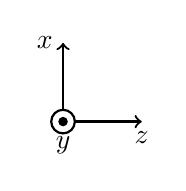
\begin{tikzpicture}
        % Draw axes
        \draw[thick,->] (1.5mm,0) -- (1,0) node[anchor=north]{$z$};
        \draw[thick,->] (0,1.5mm) -- (0,1) node[anchor=east]{$x$};
        \node at (0,-0.3) {$y$};
        % Draw origin
        % \draw[thick] (-1mm,-1mm) -- (1mm,1mm); % Diagonal line 1 for the cross
        % \draw[thick] (-1mm,1mm) -- (1mm,-1mm); % Diagonal line 2 for the cross

        \filldraw[black] (0,0) circle (1.5pt);
        \draw[thick] (0,0) circle (1.5mm);
    \end{tikzpicture}
    \caption{Coordinate System after $P_2$}
    \label{fig:3-17-2}
\end{figure}


After that, padding the reverse lens $L_1$, the $x$ and $y$ axis is reversed, so the coordinate system is shown in Figure \ref{fig:3-17-3}

\begin{figure}[H]

    \centering
    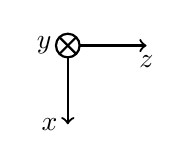
\begin{tikzpicture}
        % Draw axes
        \draw[thick,->] (1.5mm,0) -- (1,0) node[anchor=north]{$z$};
        \draw[thick,->] (0,-1.5mm) -- (0,-1) node[anchor=east]{$x$};
        \node at (-0.3,0) {$y$};
        % Draw origin
        \draw[thick] (-1mm,-1mm) -- (1mm,1mm); % Diagonal line 1 for the cross
        \draw[thick] (-1mm,1mm) -- (1mm,-1mm); % Diagonal line 2 for the cross

        % \filldraw[black] (0,0) circle (1.5pt);
        \draw[thick] (0,0) circle (1.5mm);
    \end{tikzpicture}
    \caption{Coordinate System after $L_1$}
    \label{fig:3-17-3}
\end{figure}

And then, padding the reverse lens $L_2$, the $x$ and $y$ axis is reversed again, so the coordinate system is shown in Figure \ref{fig:3-17-4}

\begin{figure}[H]
    \centering
    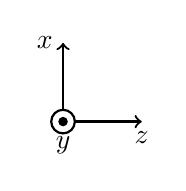
\begin{tikzpicture}
        % Draw axes
        \draw[thick,->] (1.5mm,0) -- (1,0) node[anchor=north]{$z$};
        \draw[thick,->] (0,1.5mm) -- (0,1) node[anchor=east]{$x$};
        \node at (0,-0.3) {$y$};
        % Draw origin
        % \draw[thick] (-1mm,-1mm) -- (1mm,1mm); % Diagonal line 1 for the cross
        % \draw[thick] (-1mm,1mm) -- (1mm,-1mm); % Diagonal line 2 for the cross

        \filldraw[black] (0,0) circle (1.5pt);
        \draw[thick] (0,0) circle (1.5mm);
    \end{tikzpicture}
    \caption{Coordinate System after $L_2$}
    \label{fig:3-17-4}
\end{figure}

The next step is padding the mirror $P_3$, the $x$ axis will be reversed, so the coordinate system is shown in Figure \ref{fig:3-17-5}

\begin{figure}[H]
    \centering
    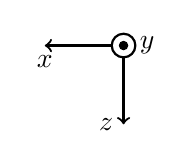
\begin{tikzpicture}
        % Draw axes
        \draw[thick,->] (-1.5mm,0) -- (-1,0) node[anchor=north]{$x$};
        \draw[thick,->] (0,-1.5mm) -- (0,-1) node[anchor=east]{$z$};
        \node at (0.3,0) {$y$};
        % Draw origin
        % \draw[thick] (-1mm,-1mm) -- (1mm,1mm); % Diagonal line 1 for the cross
        % \draw[thick] (-1mm,1mm) -- (1mm,-1mm); % Diagonal line 2 for the cross

        \filldraw[black] (0,0) circle (1.5pt);
        \draw[thick] (0,0) circle (1.5mm);
    \end{tikzpicture}
    \caption{Coordinate System after $P_3$}
    \label{fig:3-17-5}
\end{figure}

Finally, padding the mirror $P_4$, there is two times reflection, so no axis will be reversed. Therefore the coordinate system is shown in Figure \ref{fig:3-17-6}

\begin{figure}[H]
    \centering
    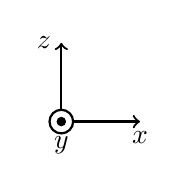
\begin{tikzpicture}
        % Draw axes
        \draw[thick,->] (1.5mm,0) -- (1,0) node[anchor=north]{$x$};
        \draw[thick,->] (0,1.5mm) -- (0,1) node[anchor=east]{$z$};
        \node at (0,-0.3) {$y$};
        % Draw origin
        % \draw[thick] (-1mm,-1mm) -- (1mm,1mm); % Diagonal line 1 for the cross
        % \draw[thick] (-1mm,1mm) -- (1mm,-1mm); % Diagonal line 2 for the cross

        \filldraw[black] (0,0) circle (1.5pt);
        \draw[thick] (0,0) circle (1.5mm);
    \end{tikzpicture}
    \caption{Coordinate System after $P_4$}
    \label{fig:3-17-6}
\end{figure}

\end{document}